\section{Artificial Neural Networks}
TODO resection

\textit{Artificial Neural Networks} (ANNs) \cite[Chapter 1]{bengio2015deep} have been used in many different applications related to artificial life and intelligence, such as robotics or machine learning.
An ANN is a directed graph structure, with vertices (referred to as neurons) and edges (referred to as connections).
This is inspired by neuroscience, with the brain consisting of neurons and synapse connections.
ANNs are useful because they consists of many discrete parts that can be individually or collectively tuned by some adaptive process,
and are easily expanded.
The \textit{universal approximation theorem} \cite{Hornik1989359} shows that relatively simple ANNs can approximate a wide variety of functions,
and the field of deep learning shows that a large complex structure with enough tuning can perform very complex tasks, such as image classification or natural language processing.

A \textit{Compositional Pattern Producing Network} (CPPN) is an \textit{artificial development encoding} introduced by Stanley in 2007 \cite{stanley-2007}.
CPPNs are structurally similar to ANNs, but differ in the use case.
Various techniques designed for ANN development and analysis may also be used for CPPNs.

A CPPN consists of a set of nodes with activation functions, weights and biases, as well as weighted connections between nodes.
Like in an ANN, external values are inputted to the first layer, then undergo transformation by weights and activation functions before being outputted by the final layer.
This can be thought of as a composition of functions producing a pattern, hence the name.
An ANN is usually structured with neurons of the same activation functions,
arranged in layers,
whereas a CPPN has few such restrictions on topology and layer-wise heterogeneity.

%The difference between an ANN and a CPPN is subtle, and is primarily in the use case.
%With ANNs there is often a subset of the possible inputs that is considered "interesting" or "valid" inputs and produce interesting or valid outputs.
%With CPPNs the user is often interested in the entire mapping of all possible inputs to output and the pattern the outputs produce.
%Another difference is in the activation function of the neurons.
%In ANNs the neuron activation function is usually the same for all neurons,
%whereas in a CPPN the network consists of a variety of functions.
%The input to the network is transformed through this composition of functions.

Figure \ref{fig:cppn} shows an example CPPN and its output when mapped over a 2D Cartesian grid.
A CPPN is able to produce a pattern without multiple steps of development,
in contrast to e.g. a CA where local interactions and time is required.
CPPNs have been used both to produce patterns for the sake of the patterns, e.g. as evolutionary art \cite{stanley2006exploiting},
but also to create patterns which are used in a larger process,
such as machine learning \cite{d2008generative} and robot control \cite{risi2013confronting}.

\begin{figure}
\centering
\begin{subfigure}[b]{.25\columnwidth}
\centering
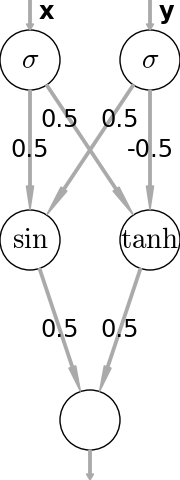
\includegraphics[width=\columnwidth]{fig/2-cppn}
\caption{~}
\end{subfigure}\hfill%
\begin{subfigure}[b]{.65\columnwidth}
\centering
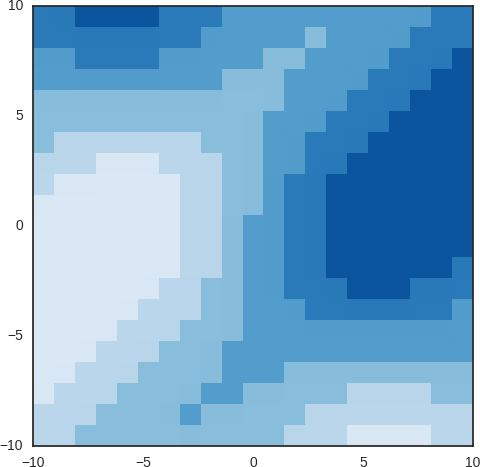
\includegraphics[width=\columnwidth]{fig/cppn_pattern}
\caption{~}
\end{subfigure}

\caption[Example CPPN]{An example composition of the sigmoid, sinusoid and hyperbolic tangent functions.
The discrete coordinates of (b) are first normalized to $[-1.0, 1.0]$ and then mapped to various output values through the CPPN (a).
%The output pattern is visualized with different shades.
%The final neuron also has an activation function, but in this case it is the identity function, so no transformation is done.
}
\label{fig:cppn}
\end{figure}

%\subsubsection{CPPNs as CA Transition Functions}
%It is possible to use a CPPN as $\Delta$.
%The CPPN takes an $\alpha$ value as input and output a $\Sigma$ value.
%In terms of memory this CPPN $\Delta$ would not scale linearly with $K^N$.
%Because the space of possible CPPN structures is unconstrained,
%the solution space is unbounded, so some intelligent search heuristic is needed in order to find good $\Delta$ for a particular problem.


\subsection{CPPNs}
TODO
